\ExamPart{Câu trắc nghiệm trả lời ngắn}{2}{}

\NQuestion Tìm số nghiệm nguyên của bất phương trình $x^2-9<0$.

\NQuestion Trong mặt phẳng tọa độ $Oxy$, cho elip $(E):\dfrac{x^2}{25}+\dfrac{y^2}{16}=1$. Tính tiêu cự của elip.

\NQuestion Từ 9 học sinh gồm 5 nam và 4 nữ, có bao nhiêu cách chọn ra 2 học sinh?

\NQuestion Một cổng vòm có dạng nửa đường tròn bán kính $5$m. Tính chiều cao của cổng tại điểm cách tâm $3$m theo phương ngang.

\begin{center}
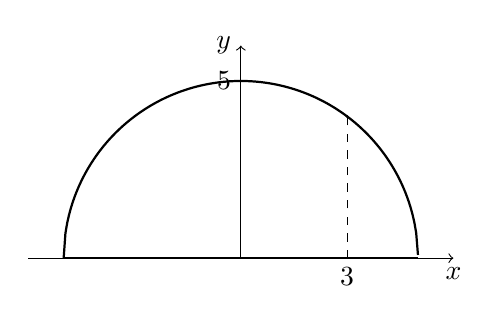
\begin{tikzpicture}[scale=0.45]
    \draw[->] (-6,0) -- (6,0) node[below] {$x$};
    \draw[->] (0,0) -- (0,6) node[left] {$y$};

    \draw[thick, domain=-5:5, samples=200] plot (\x,{sqrt(25-\x*\x)});
    \draw[thick] (-5,0) -- (5,0);

    \draw[dashed] (3,0) -- (3,4);
    \fill (3,4) circle (1.2pt);

    \node[below] at (3,0) {$3$};
    \node[left] at (0,5) {$5$};
\end{tikzpicture}

\end{center}
